% compendium/execution-market-making/market-making-models.tex
% Format pilot (2026-10-14): entries migrated from the legacy market-making blocks; dispositions
% and source checks in notes/migration.md, full derivations in
% notes/artefacts/market-making-lob/derivations.tex.

\section{Inventory risk and the price of immediacy}

\begin{qfmodel}[Grossman--Miller market making: the price of immediacy]\label{mod:grossman-miller}
\qffield{Statement} Competitive, risk-averse market makers supply immediacy to a liquidity trader who arrives before the trader with the offsetting need, and the price concession they charge compensates exactly for carrying the inventory until that trader arrives \citep[chap.~``A Primer on the Microstructure of Financial Markets'', p.~21]{crypto-cartea}. In the simplified three-date version, $n$ identical market makers, liquidity trader LT1 holding $i$ units and liquidity trader LT2 holding $-i$ units (arriving at date~2) trade an asset worth $S_3=\mu+\epsilon_2+\epsilon_3$ at date~3, and the date-1 equilibrium is \citep[same chap., pp.~23--24]{crypto-cartea}
\[ S_1=\mu-\gamma\sigma^2\,\frac{i}{n+1}, \qquad q_1^{MM}=q_1^{LT1}=\frac{i}{n+1}, \]
so LT1 sells $\frac{n}{n+1}\,i$ at once and each market maker holds $\frac{i}{n+1}$ until date~2, when LT2 arrives, the price is efficient, $S_2=\mathbb{E}[S_3\mid\epsilon_2]=\mu+\epsilon_2$, and every agent exits with zero inventory \citep[same chap., pp.~22--24]{crypto-cartea}. The liquidity discount is $\abs{S_1-\mu}=\gamma\sigma^2\abs{i}/(n+1)$; when LT1 buys ($i<0$) the market makers earn the same amount as a premium \citep[same chap., p.~24]{crypto-cartea}. Figure~\ref{fig:grossman_miller_trading} shows the holdings and trades.
\begin{figure}[H]
\centering
\scalebox{0.82}{\begin{tikzpicture}[
    >=stealth,
    thick,
    font=\small,
    every node/.style={align=center},
    price/.style={circle, fill=white, inner sep=1pt},
    flow/.style={->, gray!75}
]

% Column separators
\draw[dashed, gray!55] (0,2.65) -- (0,-2.55);
\draw[dashed, gray!55] (3.15,2.65) -- (3.15,-2.55);

% Column headers
\node at (-1.45,2.85) {$[n\times]$ MM};
\node at (1.55,2.85) {$LT1$};
\node at (4.10,2.85) {$LT2$};

% Time and inventory labels
\node at (-4.35,1.90) {$t=1$};
\node at (-4.35,0.00) {$t=2$};
\node at (-4.35,-2.00) {$t=3$};

\node at (-3.45,1.90) {$q_0^j$};
\node at (-3.45,0.00) {$q_1^j$};
\node at (-3.45,-2.00) {$q_2^j$};

% Inventory states
\node at (-1.45,1.90) {$0$};
\node at (1.55,1.90) {$i$};
\node at (4.10,1.90) {$-$};

\node at (-1.45,0.00) {$[n\times]\ \frac{i}{n+1}$};
\node at (1.55,0.00) {$\frac{i}{n+1}$};
\node at (4.10,0.00) {$-i$};

\node at (-1.45,-2.00) {$0$};
\node at (1.55,-2.00) {$0$};
\node at (4.10,-2.00) {$0$};

% Price-setting nodes
\node[price] (S1) at (0,0.95) {$S_1$};
\node[price] (S2) at (0,-1.05) {$S_2$};

% Trade labels
\node at (-2.25,0.95) {Trade};
\node at (-2.25,-1.05) {Trade};

% Date-1 trade and post-trade inventory allocation
\draw[flow] (-1.25,1.72) -- ($(S1)+(-0.18,0.15)$);
\draw[flow] (1.35,1.72) -- ($(S1)+(0.18,0.15)$);
\draw[flow] ($(S1)+(-0.18,-0.15)$) -- (-1.25,0.18);
\draw[flow] ($(S1)+(0.18,-0.15)$) -- (1.35,0.18);

% Date-2 trade and final inventory allocation
\draw[flow] (-1.25,-0.18) -- ($(S2)+(-0.18,0.15)$);
\draw[flow] (1.35,-0.18) -- ($(S2)+(0.18,0.15)$);
\draw[flow] (3.85,-0.15) -- ($(S2)+(0.22,0.05)$);
\draw[flow] ($(S2)+(-0.18,-0.15)$) -- (-1.25,-1.82);
\draw[flow] ($(S2)+(0.18,-0.15)$) -- (1.35,-1.82);
\draw[flow] ($(S2)+(0.24,-0.05)$) -- (3.85,-1.82);

\end{tikzpicture}
}
\caption{Holdings $q_t^j$ and trading in the Grossman--Miller model, after \citep[Figure~2.1, p.~23]{crypto-cartea}.}\label{fig:grossman_miller_trading}
\end{figure}

\qffield{Notation} Local override for this entry, \hyperref[res:grossman-miller-trading-fees]{the fee result} and \hyperref[res:grossman-miller-liquidity-measures]{the liquidity measures}: $\sigma^2$ is the variance of one period's value shock, in squared price units and not annualised; $\gamma$ is the coefficient of absolute risk aversion; $q_t^j$ is agent $j$'s holding on leaving date $t$, and $S_t$ the date-$t$ trade price.

\qffield{Conditions} Dates $t\in\{1,2,3\}$; shocks $\epsilon_2,\epsilon_3$ independent $N(0,\sigma^2)$, each announced between dates $t-1$ and $t$; every agent has CARA utility $U(X)=-\exp(-\gamma X)$; market makers start with no inventory; the arrival of LT2 at date~2 is certain; no trading or holding costs \citep[same chap., p.~21]{crypto-cartea}. Interpretation: the concession charges for risk, not for information; no agent is informed, which separates this model from \hyperref[mod:kyle-single-auction]{Kyle's}. Idea of the proof: solve backwards; with CARA utility and normal shocks each agent's demand is $(\mathbb{E}[\text{next price}]-\text{price})/(\gamma\sigma^2)$, and market clearing at each date gives the prices \citep[same chap., pp.~22--23]{crypto-cartea}; the full working is in the derivations artefact listed under \emph{Further reading}.

\qffield{Practice} The discount rises with the size of the liquidity need $\abs{i}$, risk aversion $\gamma$ and volatility $\sigma^2$, and falls with competition $n$; as $n$ grows the premium goes to zero, $S_1$ tends to $\mu$, and LT1's immediate trade tends to $i$ \citep[same chap., p.~24]{crypto-cartea}. Competition is itself set by participation costs: in Grossman and Miller's earlier entry stage, the number of market makers falls monotonically as the participation cost $c$ rises, which raises the discount \citep[same chap., p.~25]{crypto-cartea}. Per-share fees and two empirical liquidity measures follow from the same equilibrium: see \hyperref[res:grossman-miller-trading-fees]{trading fees} and \hyperref[res:grossman-miller-liquidity-measures]{price impact and return reversal}. Interpretation: the quoted inside spread implied by the model, a bid at $\mu-p$ and an ask at $\mu+p$ with $p=\gamma\sigma^2\abs{i}/(n+1)$, is $2p$.

\qffield{Pitfalls} The model solves a single Walrasian clearing rather than a trading mechanism \citep[same chap., pp.~26--27]{crypto-cartea}, and the offsetting trader arrives for sure; the arrival time and its uncertainty, which drive inventory risk in continuous-time quoting models, are absent. Interpretation: reading every concession as risk compensation overstates inventory costs where order flow is informed.

\qffield{See also} \hyperref[mod:kyle-single-auction]{Kyle single-auction model} (contrast: risk-neutral market makers, price impact from information); \hyperref[mod:avellaneda-stoikov]{Avellaneda--Stoikov quoting} (generalisation: inventory risk in continuous time with random order arrival); \hyperref[mod:static-limit-order-depth]{static limit-order depth} (the same immediacy supplied through posted orders).

\qffield{Further reading} \citep{grossman-miller-1988}, the original model, including participation costs (not yet read for this entry); own full derivation, from the legacy notes: \nolinkurl{notes/artefacts/market-making-lob/derivations.tex}.

\qffield{Index} Grossman--Miller; immediacy; liquidity premium; liquidity discount; inventory risk; risk transfer; dealer competition; CARA--normal equilibrium

\qffield{Status} Verification: partly checked 2026-10-14 (every formula and the comparative statics against \texttt{crypto-cartea}, pp.~21--27, read from page images of a scanned copy; the original paper not consulted). Stability: draft. Currency: timeless (theory).
\end{qfmodel}

\begin{qfresult}[Grossman--Miller with per-share trading fees]\label{res:grossman-miller-trading-fees}
\qffield{Statement} If every trader pays a fee $\eta$ per share bought or sold, the date-2 price is unchanged, $S_2=\mu+\epsilon_2$, but for a seller ($i>0$) the date-1 price falls to \citep[chap.~``A Primer on the Microstructure of Financial Markets'', pp.~25--26]{crypto-cartea}
\[ S_1=\mu-\gamma\sigma^2\,\frac{i}{n+1}-2\Big(\frac{n}{n+1}\Big)\eta, \qquad q_1^{LT1,\ast}=\frac{i}{n+1}+2\Big(\frac{n}{n+1}\Big)\frac{\eta}{\gamma\sigma^2}. \]
The initiating liquidity trader pays his own fee and, through the lower price, the fraction $n/(n+1)$ of the market makers' round-trip fees $2\eta$, and keeps more inventory after date~1 than without fees \citep[same chap., p.~26]{crypto-cartea}.

\qffield{Notation} As in \hyperref[mod:grossman-miller]{the Grossman--Miller model}.

\qffield{Conditions} The model of \hyperref[mod:grossman-miller]{the Grossman--Miller entry}, with fees proportional to shares rather than to dollar volume, positions remaining after date~2 liquidated at date~3, and desired trades large enough that every participant prefers trading to not trading \citep[same chap., p.~25]{crypto-cartea}. Idea of the proof: fees cancel at date~2 because remaining positions are sold either then or at date~3; at date~1 they reduce the market makers' demand by the round-trip fee, $q_1^{MM}=(\mu-S_1-2\eta)/(\gamma\sigma^2)$, and clearing $i=nq_1^{MM}+q_1^{LT1}$ gives the price \citep[same chap., pp.~25--26]{crypto-cartea}.

\qffield{Practice} Liquidity traders whose desired trade is small relative to the fee do not trade at all \citep[same chap., p.~25]{crypto-cartea}. Participation costs and fees act differently: participation costs work through the number of market makers, while fees work mainly through the discount and the immediacy obtained, since each market maker pays $2\eta$ per trade but recovers $2n\eta/(n+1)$ through the discount \citep[same chap., p.~26]{crypto-cartea}.

\qffield{Pitfalls} Real exchange fees are often proportional to dollar volume and differ by side and by maker or taker \citep[same chap., p.~25]{crypto-cartea}; the closed form assumes the same per-share fee for everyone.

\qffield{See also} \hyperref[mod:grossman-miller]{Grossman--Miller model} (the base case, $\eta=0$).

\qffield{Index} trading fees; exchange fees; fee incidence; participation cost; no-trade region; liquidity discount

\qffield{Status} Verification: partly checked 2026-10-14 (the formulas and fee incidence against \texttt{crypto-cartea}, pp.~25--26, from page images of a scanned copy in which several signs are faint; the printed results agree with the clearing condition on the same page). Stability: draft. Currency: timeless (theory).
\end{qfresult}

\begin{qfresult}[Grossman--Miller liquidity measures: linear price impact and negative autocovariance]\label{res:grossman-miller-liquidity-measures}
\qffield{Statement} Read as trading in a limit-order book, where LT1's market orders walk the book posted by the market makers, the Grossman--Miller date-1 price is linear in the quantity LT1 trades \citep[chap.~``A Primer on the Microstructure of Financial Markets'', pp.~26--27]{crypto-cartea}:
\[ S_1=\mu+\lambda\,q^{LT1}, \qquad \lambda=-\frac{1}{n}\,\gamma\sigma^2, \qquad q^{LT1}=i\,\frac{n}{n+1}. \]
With public news $\epsilon_1$ before LT1 trades and efficient price $\mu_t=\mathbb{E}[S_3\mid\epsilon_1,\ldots,\epsilon_t]$, the price changes $\Delta_1=S_1-S_0$ and $\Delta_2=S_2-S_1$ satisfy \citep[same chap., pp.~27--28]{crypto-cartea}
\[ \operatorname{Cov}[\Delta_1,\Delta_2]=-\lambda^2\operatorname{Var}[q^{LT1}]<0. \]

\qffield{Notation} As in \hyperref[mod:grossman-miller]{the Grossman--Miller model}; here $q^{LT1}$ is the quantity LT1 trades at date~1, not a holding, and $\lambda$ is the slope of price on that quantity.

\qffield{Conditions} The model of \hyperref[mod:grossman-miller]{the Grossman--Miller entry}, with shocks $\epsilon_1,\epsilon_2,\epsilon_3$ i.i.d.\ normal with variance $\sigma^2$, and liquidity demand independent of news \citep[same chap., pp.~27--28]{crypto-cartea}. Idea of the proof: $S_1=\mu_1+\lambda q^{LT1}$ and $S_2=\mu_2$, so the order-pressure term enters $\Delta_1$ and reverses in $\Delta_2$ \citep[same chap., p.~28]{crypto-cartea}.

\qffield{Practice} A more liquid market has a smaller $\abs{\lambda}$, from more competition, less risk aversion or lower volatility \citep[same chap., p.~27]{crypto-cartea}. As $\lambda$ goes to zero, so does the autocovariance, and the price process converges to the efficient-price martingale \citep[same chap., p.~28]{crypto-cartea}. The two measures coincide here only because the model is essentially static; in dynamic models they capture different things, permanent effects of order flow on the efficient price as against the temporary effect in each trader's execution price \citep[same chap., p.~28]{crypto-cartea}.

\qffield{Pitfalls} Interpretation: an empirical regression of price changes on signed order flow, or a negative return autocovariance, mixes this inventory effect with information and bid--ask bounce; this model alone cannot attribute it. Compare the information slope of \hyperref[mod:kyle-single-auction]{Kyle's model}.

\qffield{See also} \hyperref[mod:grossman-miller]{Grossman--Miller model} (source of the equilibrium); \hyperref[mod:kyle-single-auction]{Kyle single-auction model} (contrast: a price-impact slope from information).

\qffield{Index} price impact; Kyle's lambda (contrast); liquidity measure; autocovariance of price changes; return reversal; temporary impact; transitory price pressure

\qffield{Status} Verification: partly checked 2026-10-14 (both formulas and the comparative statics against \texttt{crypto-cartea}, pp.~26--28, from page images of a scanned copy). Stability: draft. Currency: timeless (theory).
\end{qfresult}

\section{Quoting with limit orders}

\begin{qfmodel}[Static limit-order depth with exponential fill probability]\label{mod:static-limit-order-depth}
\qffield{Statement} A small, risk-neutral market maker with costless inventory and infinite patience chooses depths $\delta^\pm$ from the midprice $S_t$ for a sell order at $S_t+\delta^+$ and a buy order at $S_t-\delta^-$; a buy (sell) market order arrives with probability $p^+$ ($p^-$) and reaches depth $\delta$ with probability $e^{-\kappa^\pm\delta}$, and expected profit per trade is maximised by \citep[chap.~``A Primer on the Microstructure of Financial Markets'', p.~29, eq.~(2.3)]{crypto-cartea}
\[ \max_{\delta^+,\delta^-}\Big\{p^+e^{-\kappa^+\delta^+}\delta^+ + p^-e^{-\kappa^-\delta^-}\delta^-\Big\}, \qquad \delta^{\pm,\ast}=\frac{1}{\kappa^\pm}. \]
The optimal depth equals the mean depth of the book on that side \citep[same chap., p.~30]{crypto-cartea}. This is a static simplification set up in place of the dynamic Ho--Stoll dealer model, which the authors give as the usual first reference \citep[same chap., p.~28]{crypto-cartea}. Figure~\ref{fig:limit_order_market_making} shows the depths and fill probabilities.
\begin{figure}[H]
\centering
\scalebox{0.86}{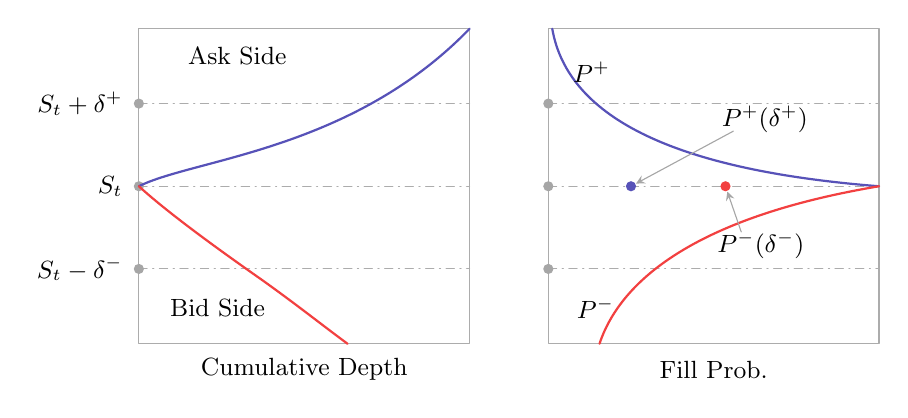
\begin{tikzpicture}[
    >=stealth,
    font=\small,
    line cap=round,
    line join=round,
    dot/.style={circle, fill=gray!70, inner sep=1.3pt},
    guide/.style={dash dot, gray!65, thin}
]

\definecolor{lobblue}{rgb}{0.34,0.32,0.72}
\definecolor{lobred}{rgb}{0.95,0.25,0.25}

% Shared price levels
\def\yask{3.05}
\def\ymid{2.00}
\def\ybid{0.95}

% Left panel: cumulative depth
\draw[gray!65] (0,0) rectangle (4.20,4.00);
\draw[guide] (0,\yask) -- (4.20,\yask);
\draw[guide] (0,\ymid) -- (4.20,\ymid);
\draw[guide] (0,\ybid) -- (4.20,\ybid);

\node[left] at (-0.08,\yask) {$S_t+\delta^+$};
\node[left] at (-0.08,\ymid) {$S_t$};
\node[left] at (-0.08,\ybid) {$S_t-\delta^-$};
\node[dot] at (0,\yask) {};
\node[dot] at (0,\ymid) {};
\node[dot] at (0,\ybid) {};

\draw[lobblue, thick] (0,\ymid)
    .. controls (0.70,2.35) and (2.70,2.45) .. (4.20,4.00);
\draw[lobred, thick] (0,\ymid)
    .. controls (0.35,1.68) and (0.95,1.24) .. (1.55,0.82)
    .. controls (2.00,0.50) and (2.35,0.22) .. (2.65,0.00);

\node at (1.25,3.65) {Ask Side};
\node at (1.00,0.45) {Bid Side};
\node at (2.10,-0.33) {Cumulative Depth};

% Right panel: fill probability
\begin{scope}[xshift=5.20cm]
\draw[gray!65] (0,0) rectangle (4.20,4.00);
\draw[guide] (0,\yask) -- (4.20,\yask);
\draw[guide] (0,\ymid) -- (4.20,\ymid);
\draw[guide] (0,\ybid) -- (4.20,\ybid);
\node[dot] at (0,\yask) {};
\node[dot] at (0,\ymid) {};
\node[dot] at (0,\ybid) {};

\draw[lobblue, thick] (0.05,4.00)
    .. controls (0.25,2.85) and (1.65,2.20) .. (4.20,\ymid);
\draw[lobred, thick] (0.65,0.00)
    .. controls (0.95,0.90) and (2.05,1.64) .. (4.20,\ymid);

\node at (0.55,3.45) {$P^+$};
\node at (0.60,0.45) {$P^-$};
\node at (2.75,2.85) {$P^+(\delta^+)$};
\node at (2.70,1.25) {$P^-(\delta^-)$};

\node[dot, fill=lobblue] (pplus) at (1.05,2.00) {};
\node[dot, fill=lobred] (pminus) at (2.25,2.00) {};
\draw[->, gray!70] (2.35,2.70) -- (pplus);
\draw[->, gray!70] (2.45,1.42) -- (pminus);

\node at (2.10,-0.33) {Fill Prob.};
\end{scope}

\end{tikzpicture}
}
\caption{Limit-order depths and probability of execution, after \citep[Figure~2.2, p.~30]{crypto-cartea}.}\label{fig:limit_order_market_making}
\end{figure}

\qffield{Notation} Local override for this entry: $p^\pm$ are probabilities of market-order arrival, not prices, and $P^\pm(\delta)$ is the probability that an arriving market order reaches depth $\delta$, not a bond or put price.

\qffield{Conditions} Everyone agrees on the value $S_t$ (no information asymmetry); other market makers' orders form a fixed book that does not react; the market maker has no inventory or trading costs and liquidates at the midprice \citep[same chap., pp.~28--29]{crypto-cartea}. Idea of the proof: the problem separates by side, and the first-order condition $p^\pm e^{-\kappa^\pm\delta^\pm}(1-\kappa^\pm\delta^\pm)=0$ gives the depth; the arrival probabilities scale profit but not the optimal depth (Interpretation, own derivation).

\qffield{Practice} The model isolates the trade-off between margin per trade and probability of execution \citep[same chap., p.~30]{crypto-cartea}; quoting deeper earns more per fill and fills less often.

\qffield{Pitfalls} The authors list what makes it unrealistic: the arrival and fill probabilities are special, constant and exogenous; the market maker's decision does not affect other traders; and the objective is static \citep[same chap., p.~30]{crypto-cartea}. Interpretation: there is no inventory penalty and no adverse selection, so the depth does not respond to position or to informed flow; \hyperref[mod:avellaneda-stoikov]{Avellaneda--Stoikov} adds inventory.

\qffield{See also} \hyperref[mod:avellaneda-stoikov]{Avellaneda--Stoikov quoting} (generalisation: dynamic, with inventory and the same exponential intensity); \hyperref[mod:grossman-miller]{Grossman--Miller model} (the immediacy this quoting supplies).

\qffield{Further reading} \citep{ho-stoll-1981}, the dynamic dealer model this simplifies (not yet read for this entry; see the pathway backlog); own full derivation, from the legacy notes: \nolinkurl{notes/artefacts/market-making-lob/derivations.tex}.

\qffield{Index} limit-order placement; quote depth; fill probability; probability of execution; exponential order-book depth; static market making; Ho--Stoll (static simplification)

\qffield{Status} Verification: partly checked 2026-10-14 (the problem, the solution and the stated limitations against \texttt{crypto-cartea}, pp.~28--30, from page images of a scanned copy; the Ho--Stoll paper not consulted). Stability: draft. Currency: timeless (theory).
\end{qfmodel}

\begin{qfmodel}[Avellaneda--Stoikov inventory-aware quotes]\label{mod:avellaneda-stoikov}
\qffield{Statement} A dealer with CARA utility, inventory $q$ and horizon $T$ quotes around a reservation (indifference) price rather than the midprice $s$ \citep[sec.~2.2, eq.~(8), p.~219]{s6-stoikov}:
\[ r(s,q,t)=s-q\gamma\sigma^2(T-t). \]
With symmetric exponential execution intensities $\lambda^a(\delta)=\lambda^b(\delta)=Ae^{-k\delta}$, an expansion of the value function in $q$ with a first-order approximation of the order-arrival terms gives the same reservation price and a bid--ask spread, independent of inventory, of \citep[sec.~3.2, eqs.~(29)--(30), p.~221]{s6-stoikov}
\[ \delta^a+\delta^b=\gamma\sigma^2(T-t)+\frac{2}{\gamma}\ln\Big(1+\frac{\gamma}{k}\Big). \]

\qffield{Notation} Local override for this entry: the midprice follows $dS_u=\sigma\,dW_u$, so $\sigma$ is an absolute volatility in price units per square root of the model's time unit, not the annualised volatility of returns; $s$ is the current midprice; $\delta^a=p^a-s$ and $\delta^b=s-p^b$ are the quote distances; $\lambda^{a}$, $\lambda^{b}$ are Poisson execution intensities, not price-impact slopes \citep[secs.~2.1 and 2.4, pp.~218--219]{s6-stoikov}.

\qffield{Conditions} Arithmetic Brownian midprice with no drift and a zero interest rate; exponential utility of terminal wealth plus inventory marked at the midprice; one-share limit orders, updated continuously at no cost, filled at Poisson rates that decrease with distance from the midprice \citep[secs.~2.1--2.4, pp.~218--219]{s6-stoikov}. The exponential intensity follows from a constant market-order frequency, a power-law order-size distribution and a logarithmic temporary impact, with $A=\Lambda/\alpha$ and $k=\alpha K$; a power-law impact gives a power-law intensity instead \citep[sec.~2.5, eq.~(12), p.~220]{s6-stoikov}. Exact quotes solve the HJB equation and two implicit equations for the distances \citep[sec.~3.1, eqs.~(15)--(19), pp.~220--221]{s6-stoikov}; the closed form above is an approximation \citep[sec.~3.2, p.~221]{s6-stoikov}. A long position ($q>0$) puts the reservation price below the midprice, so both quotes shift down to sell \citep[sec.~2.2, p.~219]{s6-stoikov}.

\qffield{Practice} In 1000 simulations with $s=100$, $T=1$, $\sigma=2$, $\gamma=0.1$, $k=1.5$, $A=140$ and $dt=0.005$, the inventory strategy earned a mean profit of 65.0 with standard deviation 6.6, against 68.4 and 12.7 for a strategy quoting the same average spread of 1.49 symmetrically around the midprice; final inventory had standard deviation 2.9 against 8.4 \citep[sec.~3.3, Table~1, p.~222]{s6-stoikov}. The symmetric strategy earns slightly more because it trades more, but its P\&L is much more dispersed \citep[sec.~3.3, p.~222]{s6-stoikov}.

\qffield{Pitfalls} Interpretation: the closed form is a control template, not a production model; real books add queue position, tick size, discrete inventory limits, latency, rebates, hedging instruments and fill probabilities that change with regime. The approximate spread does not depend on inventory only because the intensities are exponential \citep[sec.~3.2, p.~221]{s6-stoikov}. Interpretation: the formula has no inventory limit; a hard limit needs the bounded-inventory solution read in this pathway (\texttt{wide-gueant-lehalle-tapia}, not yet read).

\qffield{See also} \hyperref[mod:static-limit-order-depth]{Static limit-order depth} (special case: no inventory risk, static); \hyperref[mod:grossman-miller]{Grossman--Miller model} (the same inventory-risk premium in a three-date equilibrium).

\qffield{Further reading} Own working from the legacy notes: \nolinkurl{notes/artefacts/market-making-lob/derivations.tex}.

\qffield{Index} Avellaneda--Stoikov; reservation price; indifference price; inventory skew; optimal bid--ask spread; market making with limit orders; exponential fill intensity; HJB market making

\qffield{Status} Verification: partly checked 2026-10-14 (the reservation price, intensity, spread and simulation results against the author-hosted journal PDF of \texttt{s6-stoikov}, pp.~217--222; the HJB equation and expansion steps read but not re-derived). Stability: draft. Currency: as published in 2008; review annually with the catalogue record.
\end{qfmodel}

\section{Information and price impact}

\begin{qfmodel}[Kyle single-auction model: informed trading and linear price impact]\label{mod:kyle-single-auction}
\qffield{Statement} One risk-neutral insider who knows the asset value $v\sim N(\mu,\sigma_v^2)$, price-insensitive noise traders with net order $u\sim N(0,\sigma_u^2)$ independent of $v$, and competitive risk-neutral market makers who see only the net order flow $y=x+u$ and set $S(y)=\mathbb{E}[v\mid y]$ \citep[chap.~``A Primer on the Microstructure of Financial Markets'', pp.~31--32]{crypto-cartea} have a linear equilibrium \citep[chap.~``Strategic Trader Models I: Informed Traders'', p.~93, eqs.~(4.3)--(4.5)]{catalogue-0496}:
\[ x(v)=\beta(v-\mu), \qquad S(y)=\mu+\lambda y, \qquad \beta=\frac{\sigma_u}{\sigma_v}, \qquad \lambda=\frac{\sigma_v}{2\sigma_u}. \]
The insider's ex ante expected profit is $\tfrac12\sigma_v\sigma_u$ \citep[same chap., p.~97, eq.~(4.17)]{catalogue-0496}, and the posterior variance of $v$ after the auction is exactly half the prior, whatever the order flow: price reveals half of the insider's information \citep[same chap., p.~98, eq.~(4.20)]{catalogue-0496}.

\qffield{Notation} Source notation: \texttt{catalogue-0496} writes $p_0$ for $\mu$, $\Sigma_0$ for $\sigma_v^2$, $\sigma_\mu$ for $\sigma_u$ and $P$ for the price; \texttt{crypto-cartea} writes $\sigma$ for $\sigma_v$. Here $\lambda$ is a price-impact slope, in price per share.

\qffield{Conditions} A single auction; the insider does not observe $u$ before trading; normality of $v$ and $u$; market makers earn zero expected profit given the order flow, so price is semi-strong efficient \citep[same chap., pp.~91--92]{catalogue-0496}; \citep[chap.~``A Primer on the Microstructure of Financial Markets'', p.~32]{crypto-cartea}. There is no other linear equilibrium, but nonlinear equilibria are not excluded \citep[chap.~``Strategic Trader Models I: Informed Traders'', p.~97]{catalogue-0496}. Idea of the proof: given a linear price rule the insider's expected profit $x(v-\mu)-\lambda x^2$ is quadratic, so $\beta=1/(2\lambda)$; given a linear strategy, $v$ and $y$ are jointly normal and the projection $\mathbb{E}[v\mid y]$ is linear in $y$; the two conditions fix $\beta$ and $\lambda$ \citep[same chap., pp.~93--96]{catalogue-0496}.

\qffield{Practice} Doubling the noise-trader standard deviation doubles the insider's order and expected profit and leaves the ex ante price unchanged \citep[same chap., p.~97]{catalogue-0496}. Market makers are risk-neutral, so any premium compensates their informational disadvantage and is borne by the price-insensitive liquidity traders \citep[chap.~``A Primer on the Microstructure of Financial Markets'', p.~31]{crypto-cartea}. Interpretation (own derivation): the insider trades only part of the mispricing, because a larger order reveals more through $y$; $\lambda$ rises with $\sigma_v$ and falls with $\sigma_u$.

\qffield{Pitfalls} A linear price rule implies a negative price for a large enough sell imbalance, so it is at best an approximation of actual price behaviour \citep[chap.~``Strategic Trader Models I: Informed Traders'', p.~96]{catalogue-0496}. The joint-normality assumption drives the predictions on trade size and volume \citep[same chap., p.~98]{catalogue-0496}. The textbook account in \texttt{crypto-cartea} prints the equilibrium price as $\mu+2(x+u)\sigma_u/\sigma$, so $\lambda=2\sigma_u/\sigma$ \citep[chap.~``A Primer on the Microstructure of Financial Markets'', p.~33]{crypto-cartea}; this is the reciprocal of the value in \texttt{catalogue-0496}, eq.~(4.5), and of the value implied by its own preceding step $\beta=(2\lambda)^{-1}$. The authors' errata correct the price to $\mu+(x+u)\sigma/(2\sigma_u)$, so $\lambda=\sigma/(2\sigma_u)$, in agreement with \texttt{catalogue-0496} \citep[entries for p.~33]{crypto-cartea-errata}. Do not copy $\lambda$ from the printed page.

\qffield{See also} \hyperref[mod:grossman-miller]{Grossman--Miller model} (contrast: a premium for risk, not for information); \hyperref[res:grossman-miller-liquidity-measures]{Grossman--Miller liquidity measures} (contrast: an inventory price-impact slope).

\qffield{Further reading} \citep{s6-kyle}, the original model and its dynamic version (not yet read for this entry); own full derivation, from the legacy notes: \nolinkurl{notes/artefacts/market-making-lob/derivations.tex}.

\qffield{Index} Kyle model; Kyle's lambda; price impact; informed trading; insider; noise traders; adverse selection; semi-strong efficiency; information revelation; toxic order flow

\qffield{Status} Verification: partly checked 2026-10-14 (the equilibrium, profit and posterior variance against \texttt{catalogue-0496}, pp.~91--98, from page images of a scanned 1998 printing; the setup against \texttt{crypto-cartea}, pp.~31--33, whose printed $\lambda$ conflicts as noted under \emph{Pitfalls}; Kyle's paper not consulted; the p.~33 misprint confirmed against the authors' errata page 2026-10-15). Stability: draft. Currency: timeless (theory).
\end{qfmodel}

% Slice 2 (2026-10-15): Glosten--Milgrom and the dealer material of the legacy market-making
% section; dispositions and source checks in notes/migration.md, legacy text kept verbatim in
% notes/artefacts/market-making-lob/derivations.tex.

\section{Adverse selection and the bid--ask spread}

\begin{qfmodel}[Glosten--Milgrom sequential-trade model: spreads from adverse selection]\label{mod:glosten-milgrom}
\qffield{Statement} In a pure dealership market, investors arrive one at a time, randomly and anonymously, see the specialist's bid $b_t$ and ask $a_t$, and buy one unit at the ask, sell one unit at the bid, or leave; some arrivals are informed about the asset's future value $V$, the rest trade for liquidity reasons \citep[sec.~II, pp.~3--4]{glosten-milgrom-1983}. An arrival with information $\mathcal{F}_t$ has reservation price $Z_t=\rho_t\,\mathbb{E}[V\mid\mathcal{F}_t]$ and buys if $Z_t>a_t$, sells if $Z_t<b_t$; competitive, risk-neutral specialists with information $\mathcal{S}_t$ earn zero expected profit on each purchase and each sale, so the quotes solve \citep[p.~6]{glosten-milgrom-1983}
\[ a_t=\mathbb{E}[V\mid\mathcal{S}_t,\ Z_t>a_t], \qquad b_t=\mathbb{E}[V\mid\mathcal{S}_t,\ Z_t<b_t]. \]
Then $a_t\geq\mathbb{E}_t[V]\geq b_t$, with strict inequalities whenever informed buying above and informed selling below $\mathbb{E}_t[V]$ have positive probability: adverse selection alone produces a spread, with no inventory cost, risk aversion or monopoly power \citep[Prop.~1, pp.~7--9]{glosten-milgrom-1983}. Each transaction price is the specialist's updated expectation of $V$, so transaction prices form a martingale with respect to the specialist's and the public information \citep[Prop.~2, p.~10]{glosten-milgrom-1983}.

\qffield{Notation} $V>0$ is the asset's value, realised at a future date, with finite variance; $\rho_t$ is the arriving investor's liquidity (time-preference) parameter, with $\rho=1$ for the specialist; $\mathcal{F}_t$ and $\mathcal{S}_t$ are the information of the arrival and of the specialist; $\mathbb{E}_t$ is expectation given the information both share \citep[pp.~4--7]{glosten-milgrom-1983}. The paper writes $A_t,B_t$ for $a_t,b_t$, $F_t,S_t$ for $\mathcal{F}_t,\mathcal{S}_t$.

\qffield{Conditions} Every participant is risk-neutral with utility $\rho xV+c$ over shares $x$ and consumption $c$; $\rho$ is independent across traders and carries no information about $V$ \citep[pp.~4--5]{glosten-milgrom-1983}. Uninformed participation is exogenous; trades are single units; short positions in cash or stock cost nothing; zero profit on each side is motivated by Bertrand competition between equally informed specialists, and existence of the quotes is not shown in general \citep[pp.~4--6]{glosten-milgrom-1983}. If the specialist sees only public information, the ask is the smallest $a$ with $a\geq\mathbb{E}[V\mid\mathcal{H}_t,Z_t>a]$ and the bid the largest $b$ with $b\leq\mathbb{E}[V\mid\mathcal{H}_t,Z_t<b]$ \citep[p.~7]{glosten-milgrom-1983}. Idea of the proof of Proposition~1: conditional on a buy, the ask equals the expectation of $V$ given the buy; since buying selects arrivals whose own expectation exceeds a threshold and $\rho$ is uninformative, that conditional expectation is at least $\mathbb{E}_t[V]$ \citep[p.~8]{glosten-milgrom-1983}.

\qffield{Practice} The spread is larger, for given information, when insiders' information is finer, when the ratio of informed to uninformed arrivals rises, or when the dispersion of the uninformed liquidity parameter around its median falls \citep[Prop.~5, pp.~15--16]{glosten-milgrom-1983}. If buy and sell probabilities stay above $\theta_a,\theta_b>0$, prices converge and the root-mean-square spread over the first $k$ trades is at most $\sqrt{\operatorname{Var}(V)/(\theta_a\theta_b k)}$ \citep[Prop.~3, p.~11]{glosten-milgrom-1983}; with Poisson arrivals the average spread is then of the order of one over the square root of volume, because trades reveal information \citep[pp.~18--19]{glosten-milgrom-1983}. The specialist and the arrivals come to agree on the expected value of $V$ \citep[Prop.~4, p.~13]{glosten-milgrom-1983}. The market maker need not know which traders are informed: since well-informed traders rarely reveal themselves, dealers treat every order as possibly informed and revise prices with the side of each trade \citep[chap.~``Dealers'', pp.~288--289]{alpha-harris}. The two-point version with closed-form half-spreads is \hyperref[res:glosten-milgrom-half-spreads]{a separate result}.

\qffield{Pitfalls} If the liquidity motive is weak relative to the insiders' advantage, the zero-profit quotes may preclude trade, and the market shuts down until enough public information neutralises the insiders' advantage \citep[p.~9]{glosten-milgrom-1983}; if the bounded-probability condition fails, the spread need not shrink: the market may close, or every trade may occur at the bid \citep[p.~12]{glosten-milgrom-1983}. Proposition~5 compares spreads for given information; it does not say that stocks with more insiders have wider spreads on average, since more insiders also reveal information faster \citep[p.~17]{glosten-milgrom-1983}. The authors list unit lots, the absence of risk aversion and inventory costs, and a fixed underlying value as limitations \citep[sec.~IV, pp.~24--25]{glosten-milgrom-1983}. The locators are to the 1983 discussion paper, not the 1985 journal article that the catalogue names.

\qffield{See also} \hyperref[res:glosten-milgrom-half-spreads]{Glosten--Milgrom half-spreads} (special case: two values, closed form); \hyperref[res:glosten-milgrom-market-collapse]{market collapse} (special case: price-sensitive liquidity traders); \hyperref[res:adverse-selection-spread-component]{adverse-selection spread component} (special case: a textbook example); \hyperref[mod:kyle-single-auction]{Kyle single-auction model} (contrast: batch order flow and a strategic insider); \hyperref[mod:grossman-miller]{Grossman--Miller model} (contrast: a spread for inventory risk, without information).

\qffield{Further reading} \citep{s6-glosten}, the published version (not consulted for this entry); the legacy blocks it replaces, verbatim: \nolinkurl{notes/artefacts/market-making-lob/derivations.tex}.

\qffield{Index} Glosten--Milgrom; sequential trade model; adverse selection; bid--ask spread; informed trading; competitive specialist; zero-profit quotes; martingale prices; semi-strong efficiency; market breakdown; toxic order flow

\qffield{Status} Verification: partly checked 2026-10-15 (every statement against the scanned 1983 discussion paper, pp.~1--25, read from page images with OCR for running text; the 1985 journal version not consulted; the Harris passage from the text layer of a local copy). Stability: draft. Currency: timeless (theory).
\end{qfmodel}

\begin{qfresult}[Glosten--Milgrom half-spreads with two values]\label{res:glosten-milgrom-half-spreads}
\qffield{Statement} Let the asset's value be $V_H$ with probability $p$ and $V_L<V_H$ otherwise, let a fraction $\alpha$ of traders be informed, and let competitive risk-neutral market makers quote $a=\mu+\Delta_a$ and $b=\mu-\Delta_b$ around $\mu=\mathbb{E}[V\mid\mathcal{F}]$. Zero expected profit on each side gives the half-spreads \citep[chap.~``A Primer on the Microstructure of Financial Markets'', p.~35]{crypto-cartea}
\[ \Delta_a=\frac{\alpha p}{\alpha p+(1-\alpha)/2}\,(V_H-\mu)=\frac{V_H-\mu}{1+\frac{1-\alpha}{\alpha}\,\frac{1/2}{p}}, \qquad \Delta_b=\frac{\mu-V_L}{1+\frac{1-\alpha}{\alpha}\,\frac{1/2}{1-p}}. \]
With trading over time, $p_t=\mathbb{P}(V=V_H\mid\mathcal{F}_t)$ and $\mu_t=\mathbb{E}[V\mid\mathcal{F}_t]$ are updated by Bayes' rule from the order flow, the same formulas hold with $p_t,\mu_t$, and each execution price equals the expected value given the history and the side of the trade, so the price at execution times is a martingale \citep[same chap., p.~36]{crypto-cartea}.

\qffield{Notation} Local override for this entry and \hyperref[res:glosten-milgrom-market-collapse]{market collapse}: $p$ is the probability of the high value, not a price; $\alpha$ is the fraction of informed traders; $\Delta_a,\Delta_b$ are the ask and bid half-spreads; $\mathcal{F}$ is public information, including the order flow. Source notation: \texttt{crypto-cartea} writes $v$ for $V$.

\qffield{Conditions} A simplified, essentially static version of the model: one-unit orders; informed traders know $V$ and buy one unit if $a<V_H$ and $V=V_H$, sell one unit if $b>V_L$ and $V=V_L$; liquidity traders are price-insensitive and buy or sell with probability $\tfrac12$ each, whatever the value; market makers are risk-neutral, carry inventory at no cost and compete to zero expected profit, using only public information \citep[same chap., pp.~34--35]{crypto-cartea}. Idea of the proof: a buy comes from a liquidity trader with weight $(1-\alpha)/2$, who pays $\Delta_a$, and from an informed trader with weight $\alpha p$, who costs $V_H-\mu-\Delta_a$; setting the weighted profit to zero gives $\Delta_a$, and the bid is symmetric \citep[same chap., p.~35]{crypto-cartea}.

\qffield{Practice} Reading asymmetric information as toxicity, $\alpha$ is its prevalence, and $p$ with $V_H-\mu$, or $1-p$ with $\mu-V_L$, its magnitude on the buy or sell side; market makers widen each half-spread as the prevalence and magnitude of toxicity on that side rise \citep[same chap., pp.~35--36]{crypto-cartea}. Interpretation (own derivation): as $\alpha\to0$ both half-spreads vanish, and as $\alpha\to1$ the quotes reach $V_H$ and $V_L$, where only informed traders would trade.

\qffield{Pitfalls} This is a textbook simplification: the paper allows a general value distribution and price-sensitive uninformed traders \citep[sec.~II, pp.~3--6]{glosten-milgrom-1983}. With price-insensitive liquidity traders a monopolist would quote $a=V_H$, $b=V_L$; the formulas rely on competition between market makers \citep[chap.~``A Primer on the Microstructure of Financial Markets'', p.~35]{crypto-cartea}.

\qffield{See also} \hyperref[mod:glosten-milgrom]{Glosten--Milgrom model} (generalisation); \hyperref[res:glosten-milgrom-market-collapse]{market collapse} (extension: price-sensitive liquidity traders); \hyperref[res:adverse-selection-spread-component]{adverse-selection spread component} (contrast: a parametrisation by the dealer's pricing error).

\qffield{Index} Glosten--Milgrom half-spread; ask half-spread; bid half-spread; toxicity; prevalence of informed trading; Bayesian quote updating; zero-profit market making

\qffield{Status} Verification: partly checked 2026-10-15 (the setup, both formulas, the dynamic version and the interpretation against \texttt{crypto-cartea}, pp.~34--36, read from page images of a scanned copy; the zero-profit algebra re-derived). Stability: draft. Currency: timeless (theory).
\end{qfresult}

\begin{qfresult}[Glosten--Milgrom with price-sensitive liquidity traders: market collapse]\label{res:glosten-milgrom-market-collapse}
\qffield{Statement} If liquidity trader $i$ trades only when the half-spread is at most his urgency $c_i$, with $c_i$ distributed with cumulative distribution function $F$ across liquidity traders, the zero-profit half-spreads are defined implicitly by \citep[chap.~``A Primer on the Microstructure of Financial Markets'', p.~37]{crypto-cartea}; \citep[entry for p.~37]{crypto-cartea-errata}
\[ \Delta_a=\frac{V_H-\mu}{1+\frac{1-\alpha}{\alpha}\,\frac{(1-F(\Delta_a))/2}{p}}, \qquad \Delta_b=\frac{\mu-V_L}{1+\frac{1-\alpha}{\alpha}\,\frac{(1-F(\Delta_b))/2}{1-p}}. \]
Widening a half-spread drives out liquidity traders; if urgency is small, the only solutions may be the extreme ones, $\Delta_a=V_H-\mu$ and $\Delta_b=\mu-V_L$: the market collapses, only informed traders, who are then indifferent, might trade, and any trade reveals the value \citep[chap.~``A Primer on the Microstructure of Financial Markets'', p.~37]{crypto-cartea}.

\qffield{Notation} As in \hyperref[res:glosten-milgrom-half-spreads]{the two-value half-spreads}; $c_i$ is the cash-equivalent gain to liquidity trader $i$ from completing the desired trade.

\qffield{Conditions} The two-value model of \hyperref[res:glosten-milgrom-half-spreads]{the half-spreads entry}, with only the fraction $1-F(\Delta)$ of would-be liquidity buyers or sellers trading at half-spread $\Delta$ \citep[same chap., p.~37]{crypto-cartea}. ``Small'' urgency means that no liquidity trader's urgency exceeds the expected value of the asset: $F(\mu-\epsilon)=1$ for some $\epsilon>0$ \citep[same chap., p.~37, n.~5]{crypto-cartea}.

\qffield{Practice} The paper gives the same mechanism: when the proportion of insiders is high or the liquidity motive of the uninformed weak, the zero-profit quotes can preclude trade, a lemons problem as in Akerlof, and the market reopens when public information neutralises the insiders' advantage \citep[pp.~9 and~17]{glosten-milgrom-1983}.

\qffield{Pitfalls} The book prints $F(\Delta_a)$ in the bid formula; the authors' errata correct it to $F(\Delta_b)$, as given above \citep[entry for p.~37]{crypto-cartea-errata}. Do not copy the bid formula from the printed page.

\qffield{See also} \hyperref[res:glosten-milgrom-half-spreads]{Glosten--Milgrom half-spreads} (the price-insensitive case, $F\equiv0$); \hyperref[mod:glosten-milgrom]{Glosten--Milgrom model} (generalisation, with market shutdown).

\qffield{Index} market collapse; market breakdown; market shutdown; lemons problem; price-sensitive liquidity traders; urgency; liquidity dry-up; adverse selection

\qffield{Status} Verification: partly checked 2026-10-15 (the formulas, the collapse condition and its footnote against \texttt{crypto-cartea}, p.~37, from page images of a scanned copy; the correction against the authors' errata page, read from the equation source of the page; the shutdown passages against the 1983 discussion paper). Stability: draft. Currency: timeless (theory).
\end{qfresult}

\begin{qfresult}[Adverse-selection spread component: information and accounting views]\label{res:adverse-selection-spread-component}
\qffield{Statement} In a simple example based on the Glosten--Milgrom model, a dealer believes that the security is worth $V$ unconditionally, that the next trader is equally likely to buy or sell and is informed with probability $\alpha$, and that it is worth $V+e$ if an informed trader buys and $V-e$ if an informed trader sells \citep[chap.~``Bid/Ask Spreads'', p.~320]{alpha-harris}. Information view: conditional on a buy the dealer's value estimate is $(1-\alpha)V+\alpha(V+e)=V+\alpha e$, conditional on a sell $V-\alpha e$, so the adverse-selection component is $2\alpha e$ \citep[same chap., p.~320]{alpha-harris}. Accounting view: expected profit on the next trade is $\tfrac12(a-b)-\alpha e$, so breaking even requires $a-b=2\alpha e$ \citep[same chap., pp.~320--321]{alpha-harris}. Both views give the same component \citep[same chap., p.~300]{alpha-harris}.

\qffield{Notation} Source notation: Harris writes $P$ for $\alpha$, $E$ for $e$ (the dealer's pricing error when the trader is informed), and $A$, $B$ for $a$, $b$.

\qffield{Conditions} Normal costs of doing business are ignored; the example assumes that dealers know the value when informed traders trade, which the result does not need \citep[same chap., pp.~300 and~320]{alpha-harris}. The two views agree when the loss from trading with an informed trader equals the pricing error, as when the dealer cannot restore inventory before prices adjust; if the dealer can rebalance but does not recognise the informed trade, informed traders keep trading with him until the price adjusts, and his cumulative loss is still the original pricing error \citep[same chap., p.~302]{alpha-harris}. Low barriers to entry and competition from public limit orders, which undercut wide dealer quotes, limit monopoly spreads \citep[same chap., p.~298]{alpha-harris}; in a competitive dealer market free entry and exit drive dealers to normal profits, so the total spread is this component plus a transaction-cost component that covers operating costs, financing, any monopoly profit and any premium for inventory risk \citep[same chap., pp.~298--299]{alpha-harris}.

\qffield{Practice} The component rises with the probability that the next trader is informed, with the materiality of the information and with trade size, because dealers believe large traders are often well informed \citep[chap.~``Dealers'', pp.~289--291 and~295]{alpha-harris}. Price changes from the adverse-selection component are permanent, while the transaction-cost component causes bid--ask bounce \citep[chap.~``Bid/Ask Spreads'', pp.~299--300]{alpha-harris}. Volatile instruments have wider spreads, both through inventory risk for risk-averse dealers and as a proxy for asymmetric information \citep[same chap., pp.~312--313]{alpha-harris}.

\qffield{Pitfalls} This is a textbook example, not the Glosten--Milgrom paper, whose quotes are expectations conditional on a trade at the quote (\hyperref[mod:glosten-milgrom]{the model}); the legacy note that attributed $a=V+\alpha e$, $b=V-\alpha e$ to Glosten and Milgrom followed this example. The accounting view fixes only the width $a-b$; the level $V\pm\alpha e$ comes from the information view (Interpretation). Harris prints the dealer's profit against an informed buyer as $A-(V-E)$; his stated result requires $A-(V+E)$ \citep[chap.~``Bid/Ask Spreads'', p.~321]{alpha-harris}.

\qffield{See also} \hyperref[mod:glosten-milgrom]{Glosten--Milgrom model} (generalisation); \hyperref[res:glosten-milgrom-half-spreads]{Glosten--Milgrom half-spreads} (contrast: a parametrisation by the value distribution); \hyperref[meth:dealer-quote-adjustment]{dealer quote adjustment} (practice: how dealers set and revise quotes).

\qffield{Further reading} The legacy blocks it replaces, verbatim: \nolinkurl{notes/artefacts/market-making-lob/derivations.tex}.

\qffield{Index} adverse selection spread component; permanent spread component; transaction cost spread component; transitory spread component; Glosten--Milgrom theorem (Harris); information view; accounting view; spread decomposition; bid--ask bounce

\qffield{Status} Verification: partly checked 2026-10-15 (the example, both derivations, the conditions and the spread determinants against the text layer of a local copy of \texttt{alpha-harris}, 2002 Oxford printing, pp.~289--302, 312--313 and 320--321; p.~321 also from its page image). Stability: draft. Currency: timeless (theory).
\end{qfresult}

\section{Dealer inventory and quote adjustment}

\begin{qfdefinition}[Dealer inventory imbalance and the two inventory risks]\label{def:dealer-inventory-risk}
\qffield{Statement} A dealer's \emph{target inventory} is the position it wants to hold, and its \emph{inventory imbalance} is actual inventory minus target \citep[chap.~``Dealers'', p.~283]{alpha-harris}. Dealers face two inventory risks, distinguished by whether future price changes are correlated with the imbalance \citep[same chap., p.~285]{alpha-harris}:
\begin{itemize}
\item \emph{diversifiable inventory risk}: price changes independent of the imbalance; gains and losses are equally likely, they do not cause losses in the long run, and dealing in many instruments reduces their effect on total profit \citep[same chap., pp.~285--286]{alpha-harris};
\item \emph{adverse-selection risk}: price changes inversely correlated with the imbalance, because informed traders take the side their information favours, make order flow one-sided and push the dealer's inventory away from target before prices move \citep[same chap., p.~286]{alpha-harris}.
\end{itemize}

\qffield{Conditions} If long and short positions are equally costly, a dealer that does not also speculate, hedge or invest has a target of zero; where shorting costs more, targets are positive; speculating dealers set targets by their views \citep[same chap., pp.~283--284]{alpha-harris}. Large imbalances are costly to finance and expose the dealer to losses if prices move, and an imbalance beyond the dealer's capital forces liquidation \citep[same chap., p.~284]{alpha-harris}.

\qffield{Practice} Dealers avoid both risks by keeping inventory under control, so most attend to \emph{market values}, the prices that produce two-sided order flow, more than to fundamental values, which they discover as a by-product \citep[same chap., pp.~286--287]{alpha-harris}. Adverse selection is still the most important determinant of dealer profitability \citep[same chap., p.~286]{alpha-harris}.

\qffield{Pitfalls} ``Diversifiable'' here means unrelated to the dealer's imbalance; within one instrument it is still a risk that a risk-averse dealer is paid to bear, as in \hyperref[mod:grossman-miller]{Grossman--Miller} (Interpretation). A falling inventory after buys does not by itself say which risk is present; separating them needs the subsequent price path (Interpretation).

\qffield{See also} \hyperref[meth:dealer-quote-adjustment]{dealer quote adjustment} (how dealers control the imbalance); \hyperref[mod:grossman-miller]{Grossman--Miller model} (a model of the first risk); \hyperref[mod:glosten-milgrom]{Glosten--Milgrom model} (a model of the second).

\qffield{Further reading} The legacy blocks it replaces, verbatim: \nolinkurl{notes/artefacts/market-making-lob/derivations.tex}.

\qffield{Index} inventory imbalance; target inventory; inventory risk; diversifiable inventory risk; adverse selection risk; market value; fundamental value; dealer risk management

\qffield{Status} Verification: partly checked 2026-10-15 (against the text layer of a local copy of \texttt{alpha-harris}, 2002 Oxford printing, pp.~283--287). Stability: draft. Currency: timeless (concepts).
\end{qfdefinition}

\begin{qfmethod}[Dealer quote adjustment for inventory and suspected informed trading]\label{meth:dealer-quote-adjustment}
\qffield{Statement} Dealers control inventory and adverse selection with four levers: the level of both quotes, their skew, the width of the spread and the sizes shown.
\begin{enumerate}
\item \emph{Inventory.} To reduce inventory, lower bid and ask, decrease the bid size and raise the ask size; to increase it, do the opposite; an impatient dealer can take another trader's offer or hit another trader's bid, or hedge with a correlated instrument \citep[chap.~``Dealers'', pp.~284--285, Table~13-2]{alpha-harris}.
\item \emph{After a suspected informed trade.} After selling to a suspected well-informed buyer, raise the ask and lower its size to discourage further informed buying, raise the bid and its size to rebuild inventory, or buy at another trader's ask or buy a correlated instrument; after buying from a suspected informed seller, do the reverse \citep[same chap., pp.~287--288, Table~13-3]{alpha-harris}.
\item \emph{Before the next trade.} Set the ask at the value expected if the next trader buys and the bid at the value expected if the next trader sells, adjusting more when informed trading is more likely and the information more material \citep[same chap., pp.~288--290]{alpha-harris}; see \hyperref[res:adverse-selection-spread-component]{the adverse-selection component}.
\item \emph{Size.} Avoid displaying large size, so that traders must ask for it and reveal themselves \citep[same chap., p.~291]{alpha-harris}.
\end{enumerate}

\qffield{Conditions} Dealers rarely know who is informed: informed traders hide behind brokers and claim to be uninformed, and rules of thumb (large, active, impatient traders are often informed; small retail traders rarely) are useful but unreliable, so every order is treated as possibly informed \citep[same chap., pp.~288--289]{alpha-harris}. Spreads widen with asymmetric information, volatility and weak utilitarian trading interest \citep[chap.~``Bid/Ask Spreads'', pp.~312--313]{alpha-harris}.

\qffield{Practice} Searching for prices that bring two-sided order flow is price discovery: it finds market values \citep[chap.~``Dealers'', p.~284]{alpha-harris}. Demanding liquidity to rebalance gives a negative realised spread \citep[same chap., p.~284]{alpha-harris}. After a buy, raising quotes is right if the buyer was informed and a mistake if not, when value traders sell to the dealer and realised spreads fall; doing nothing is the reverse; buying at another trader's ask may limit losses against an informed buyer but is a big mistake against an uninformed one \citep[same chap., pp.~291--292, Table~13-4]{alpha-harris}. Poorly informed dealers more often mistake uninformed for informed clients, so they turn inventory quickly and earn smaller realised spreads; well-informed dealers can hold larger positions longer and earn larger realised spreads \citep[same chap., pp.~292--294]{alpha-harris}. Value traders trade when prices diverge from fundamental value, often after such mistakes or after risk-averse dealers obtain large concessions for taking big positions, and in doing so restore dealers' inventories \citep[same chap., pp.~291 and~294]{alpha-harris}. Some dealers avoid informed traders by trading only with retail or known clients, refusing anonymous size, or slicing large orders over time, which lets them offer more liquidity to the flow they accept \citep[same chap., pp.~290--291]{alpha-harris}.

\qffield{Pitfalls} Informed traders can bluff, sending small orders on one side to move a dealer before trading on the other; against traders they cannot identify, dealers should adjust prices at the same rate per quantity whatever the side, speed, size or sequence of orders \citep[same chap., pp.~292 and~294]{alpha-harris}. Interpretation: refusing flow protects the dealer but reduces the immediacy available to others; one-sided flow turns dealing into warehousing risk. These are heuristics without an objective function; \hyperref[mod:avellaneda-stoikov]{Avellaneda--Stoikov} derives the inventory skew from one.

\qffield{See also} \hyperref[def:dealer-inventory-risk]{dealer inventory risk} (prerequisite); \hyperref[res:adverse-selection-spread-component]{adverse-selection spread component} (the spread set before the next trade); \hyperref[mod:avellaneda-stoikov]{Avellaneda--Stoikov quoting} (a model of the inventory skew); \hyperref[mod:glosten-milgrom]{Glosten--Milgrom model} (a model of the revision after each trade).

\qffield{Further reading} The legacy text it replaces, tables included, is kept verbatim in \nolinkurl{notes/artefacts/market-making-lob/derivations.tex}.

\qffield{Index} inventory control; quote skew; quote shading; quote size; dealer tactics; price discovery; market value; realised spread; informed-trader identification; refusing flow; value traders; bluffing; toxic flow

\qffield{Status} Verification: partly checked 2026-10-15 (every step and table summary against the text layer of a local copy of \texttt{alpha-harris}, 2002 Oxford printing, pp.~283--294 and 312--313). Stability: draft. Currency: timeless (practice description from 2002; venue examples dated).
\end{qfmethod}
